% =====================================================================
% SecureForge Web — artigo SBC (pronto para Overleaf)
% Compilar no Overleaf: XeLaTeX ou pdfLaTeX (recomendado: pdfLaTeX)
% Estrutura: main.tex + figures/ + references.bib
% =====================================================================
\documentclass[12pt]{article}

\usepackage{sbc-template}
\usepackage{graphicx}
\usepackage{url}
\usepackage[utf8]{inputenc}
\usepackage[T1]{fontenc}
\usepackage[brazil,english]{babel}
\usepackage{booktabs}
\usepackage{tabularx}
\usepackage{multirow}
\usepackage{amsmath}
\usepackage{hyperref}

\graphicspath{{figures/}}

\title{SecureForge Web: Uma Plataforma de Diagnóstico e Hardening de Aplicações Web com Checklist OWASP e Evidências Automatizadas}

\author{
  Autores a serem preenchidos\\
  Instituição / Projeto Integrador --- Trilha AppHardener\\
  \email{contato@exemplo.edu.br}
}

\begin{document}

\maketitle

\begin{abstract}
SecureForge Web is a web platform for guided security assessment and gradual hardening of web applications. Unlike professional vulnerability scanners, it combines an OWASP/ASVS-aligned checklist, human-in-the-loop validation, and assisted automation through HTTP header inspection, static repository analysis, and a per-user AI assistant. The tool records structured evidence per checklist item, generates findings with remediation guidance, tracks security posture over time, and exports PDF reports. We describe its architecture, assessment modules, and an experimental evaluation on two applications (OWASP Juice Shop and SecureForge Web itself), demonstrating end-to-end operation from registration to posture benchmarking.
\end{abstract}

\begin{resumo}
A SecureForge Web é uma plataforma web para diagnóstico guiado e fortalecimento gradual (\emph{hardening}) de aplicações web. Diferentemente de scanners profissionais de vulnerabilidades, combina checklist alinhado a OWASP/ASVS, validação humana no fluxo e automação assistida por inspeção de headers HTTP, análise estática de repositório Git e assistente de IA configurável por usuário. A ferramenta registra evidências estruturadas por item de checklist, gera achados com recomendações de correção, acompanha a postura de segurança ao longo do tempo e exporta relatórios em PDF. Descrevemos sua arquitetura, módulos de avaliação e uma avaliação experimental sobre duas aplicações reais --- OWASP Juice Shop e a própria SecureForge Web --- demonstrando operação ponta a ponta desde o cadastro até o benchmark de postura.
\end{resumo}

\section{Introdução}
A segurança de aplicações web permanece entre as principais preocupações de equipes de desenvolvimento, laboratórios acadêmicos e pequenas organizações que não dispõem de processos formais de revisão de postura nem de ferramentas \emph{enterprise} de análise contínua~\cite{owasp-samm}. Nesse contexto, muitas equipes conhecem recomendações genéricas --- como as do OWASP Top~10 e do \emph{Application Security Verification Standard}~\cite{owasp-asvs-2021} ---, mas enfrentam dificuldade para transformá-las em um fluxo operacional repetível, rastreável e orientado à correção.

Ferramentas de \emph{Dynamic Application Security Testing}~\cite{owasp-dast} e análise estática profissional oferecem automação em escala, porém frequentemente produzem grandes volumes de alertas, exigem curva de aprendizado elevada e não integram, de forma natural, o registro de decisões humanas, priorização de \emph{hardening} e acompanhamento evolutivo da postura. Por outro lado, planilhas e documentos isolados carecem de rastreabilidade, evidência técnica e consolidação de métricas.

Este artigo apresenta a SecureForge Web\footnote{Código e documentação: \url{https://github.com/secureforgeweb/secureforgeweb}.}, uma plataforma desenvolvida no âmbito da trilha AppHardener do Projeto Integrador em Ferramentas de Segurança Aplicada. A ferramenta atua como assistente guiado: o analista cadastra uma aplicação, percorre um checklist de 24 controles organizados em categorias OWASP, recebe sugestões automáticas assistidas (HTTP, Git e IA), valida manualmente cada item, documenta evidências e consolida achados com recomendações de \emph{hardening}. O administrador pode, ainda, comparar posturas entre análises e modelos de IA utilizados por diferentes operadores.

A contribuição deste trabalho é tripla: (i)~propor um fluxo acadêmico-prático que une checklist, automação assistida e validação humana; (ii)~apresentar uma arquitetura monolítica modular implementada com tecnologias web contemporâneas; e (iii)~demonstrar a geração de evidências estruturadas por item, incluindo trechos de código, headers HTTP e resumos de varredura, persistidos para revisão posterior e exportação.

\section{Trabalhos Relacionados}
A literatura sobre segurança de aplicações web abrange desde padrões normativos e metodologias de teste até plataformas automatizadas de varredura e modelos quantitativos de postura. Esta seção posiciona a SecureForge Web em relação a esses trabalhos.

\subsection{Padrões OWASP e checklists de hardening}
O OWASP ASVS~\cite{owasp-asvs-2025} estabelece requisitos técnicos verificáveis para aplicações web, enquanto o \emph{Web Security Testing Guide}~\cite{owasp-wstg} orienta testes de segurança de forma metodológica. Esses artefatos definem \emph{o que} verificar, mas não oferecem, por si só, um fluxo operacional integrado de cadastro de aplicações, \emph{wizard} guiado, gestão de achados e relatório consolidado --- lacuna que a SecureForge Web endereça.

\subsection{Avaliação quantitativa baseada em ASVS}
Wen e Katt~\cite{wen-katt-2021} propõem modelo quantitativo de avaliação de segurança web fundamentado no ASVS. Revniuk et al.~\cite{revniuk-2023} descrevem sistema de informação para avaliação quantitativa ASVS com pesos de especialistas e visualização de resultados, arquiteturalmente próximo ao \emph{dashboard} de postura da SecureForge Web. A diferença central da proposta aqui apresentada é combinar \emph{score} de postura com automação assistida (HTTP, Git e IA) e validação humana explícita no \emph{wizard}.

\subsection{Automação, DAST e ferramentas de hardening}
Ferramentas DAST, como o OWASP ZAP~\cite{owasp-zap}, automatizam a descoberta de vulnerabilidades em escala, porém tendem a produzir alto volume de alertas. Projetos recentes aproximam-se da automação parcial~\cite{lee-2024,rodriguez-2025}, mas não integram checklist guiado por item, evidências rastreáveis por resposta, assistente de IA configurável por usuário e \emph{benchmark} administrativo entre operadores.

\subsection{Posicionamento}
Modelos de maturidade como o OWASP SAMM~\cite{owasp-samm} avaliam a capacidade organizacional de segurança de software, não o \emph{hardening} pontual de uma aplicação específica. A SecureForge Web ocupa nicho complementar: ferramenta operacional para equipes pequenas, laboratórios e projetos acadêmicos.

\section{Arquitetura do SecureForge Web}
O SecureForge Web é um monólito modular \emph{full-stack} voltado à avaliação de postura de segurança de aplicações web alinhada a checklists OWASP. A solução concentra interface, API e lógica de avaliação no mesmo pacote (\texttt{secureforgeweb\_web/}), com persistência em PostgreSQL e integrações externas sob demanda.

No lado do cliente, a SPA em React~19 (Vite~7, TypeScript, Tailwind, TanStack Query e cliente tRPC) oferece o fluxo de registro de aplicações, \emph{wizard} de checklist, \emph{findings}, \emph{dashboards} e área administrativa. No centro da arquitetura está a API Node.js~22 com Express e tRPC: autenticação (JWT em \emph{cookie}, RBAC), CRUD de domínio, geração de PDF e os assessores executados no mesmo processo da requisição (HTTP/HTTPS, \texttt{git clone} raso e LLM opcional). A persistência fica no PostgreSQL~16, acessado via Drizzle ORM.

\begin{figure}[!ht]
  \centering
  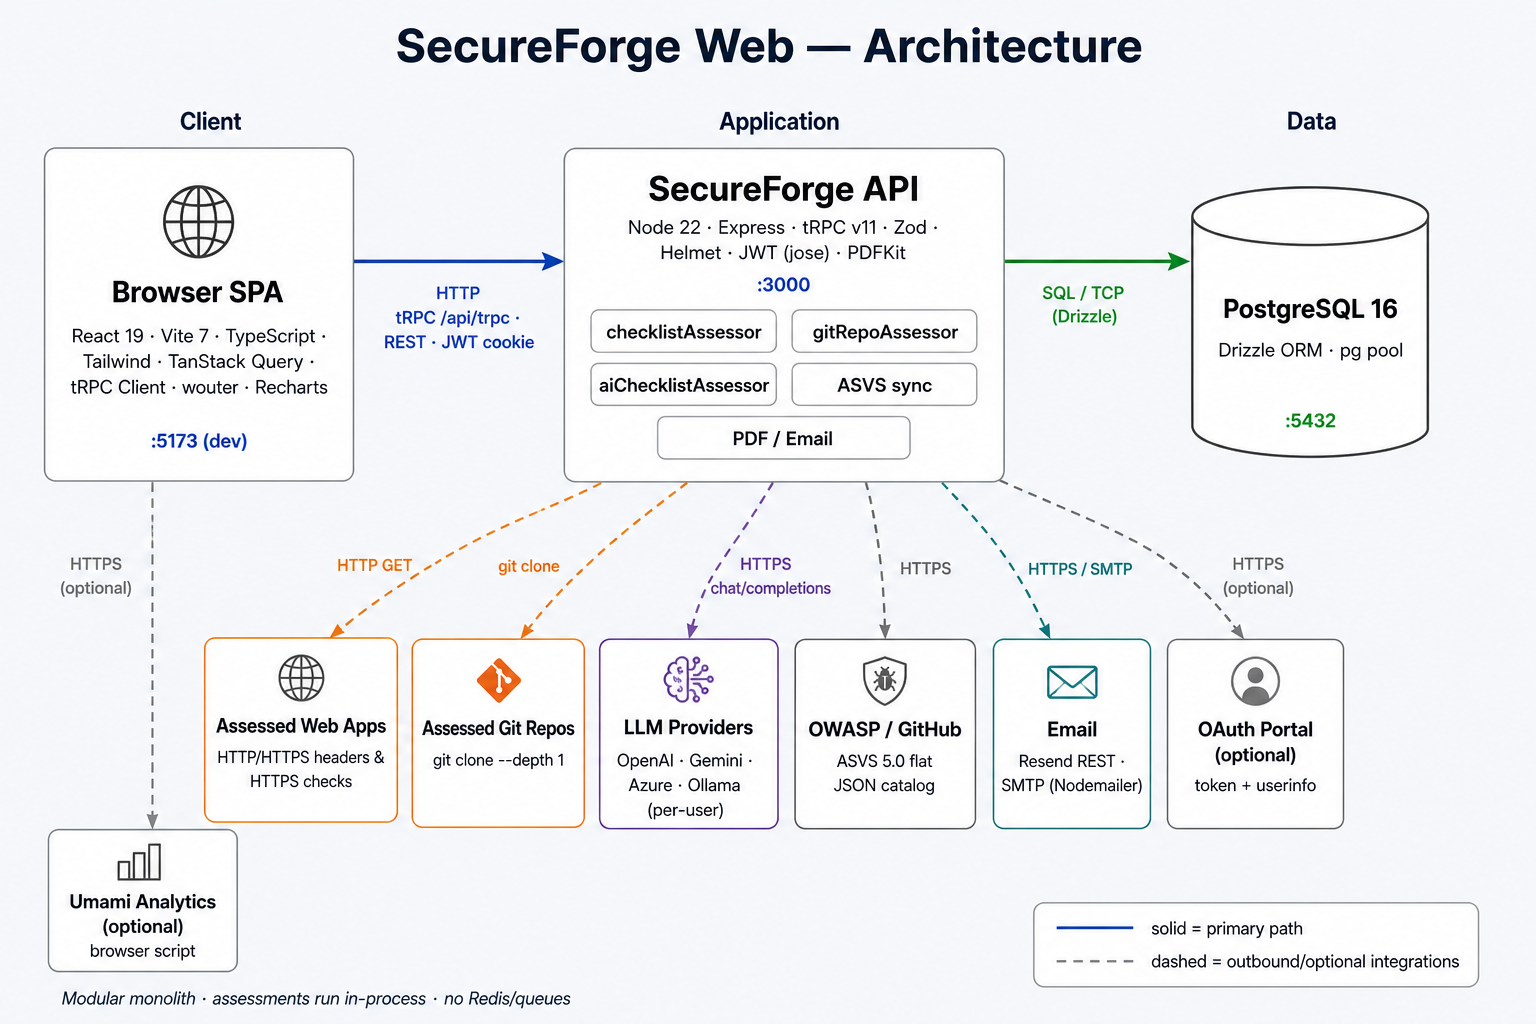
\includegraphics[width=\linewidth]{fig-architecture.png}
  \caption{Arquitetura do SecureForge Web: SPA React, API Express/tRPC, PostgreSQL e integrações (alvos HTTP/Git, LLMs, OWASP/GitHub, e-mail).}
  \label{fig:arquitetura}
\end{figure}

Ao redor do núcleo, as integrações \emph{outbound} incluem aplicações-alvo (HTTP GET), repositórios Git sob avaliação, provedores de LLM configuráveis por usuário (OpenAI, Gemini, Azure, Ollama/\emph{custom}), catálogo OWASP ASVS~5.0 via GitHub, e-mail transacional (Resend ou SMTP) e, de forma opcional, portal OAuth e analytics Umami.

\section{Limitações}
Apesar dos benefícios apresentados, a SecureForge Web possui restrições deliberadas, coerentes com o recorte acadêmico da trilha AppHardener: (1)~não substitui DAST profissional, \emph{pentest} ou varredura de dependências em produção; (2)~análise Git limita-se a repositórios acessíveis por HTTPS público, com teto de arquivos e tamanho por arquivo; (3)~heurísticas estáticas podem gerar falsos positivos/negativos; (4)~o LLM depende de chave válida e pode alucinar --- o \emph{fallback} heurístico mitiga, mas não elimina o risco; (5)~evidências refletem \emph{snapshot} no momento da execução; (6)~\emph{benchmark} administrativo compara postura agregada, não latência ou custo de API por item.

\section{Avaliação Experimental}
\subsection{Ambiente e metodologia}
A avaliação foi conduzida em ambiente de desenvolvimento local, com PostgreSQL~16 em contêiner Docker, Node.js~22 e \texttt{pnpm}. Foram cadastradas e analisadas \textbf{duas aplicações-alvo}, ambas com o \textbf{Checklist Essential SecureForge v1.0} (24 itens / 9 categorias):

\begin{enumerate}
  \item \textbf{OWASP Juice Shop} --- aplicação intencionalmente vulnerável de referência; repositório \url{https://github.com/juice-shop/juice-shop.git}; análise concluída em 15/07/2026.
  \item \textbf{SecureForge Web} (autoavaliação) --- a própria plataforma; evolução em três medições: baseline HTTP (\texttt{http://localhost:5173}, 22--23/07/2026), demonstração TLS (\texttt{https://localhost:5173}, 23/07/2026) e pós-remediação com URL da API (\texttt{https://localhost:3000}) e repositório público em 24/07/2026.
\end{enumerate}

O protocolo experimental compreendeu: (i)~configuração do assistente de IA por usuário (OpenAI \texttt{gpt-4o-mini}, teste de conexão bem-sucedido); (ii)~cadastro da aplicação (URL e/ou Git); (iii)~criação de análise e percurso do \emph{wizard} até 24/24 itens; (iv)~geração automática de achados; (v)~inspeção de \emph{dashboard}, lista de achados, acompanhamento e notificações; (vi)~exportação do relatório PDF; (vii)~no alvo SecureForge, ciclo adicional de \emph{hardening} dos achados críticos/altos e reavaliação.

\subsection{Resultados}
A Tabela~\ref{tab:comparativo} consolida as métricas oficiais de postura. O \emph{score} corresponde à proporção de itens \emph{conformes}~+~N/A sobre o checklist de 24 itens; a taxa de resolução mede achados resolvidos~+~aceitos.

\begin{table}[!ht]
\centering
\caption{Comparativo de postura: OWASP Juice Shop vs.\ SecureForge Web após hardening (Checklist Essential v1.0).}
\label{tab:comparativo}
\begin{tabular}{lrr}
\toprule
\textbf{Indicador} & \textbf{Juice Shop} & \textbf{SecureForge Web} \\
\midrule
Data da análise & 15/07/2026 & 24/07/2026 \\
Progresso do checklist & 24/24 (100\%) & 24/24 (100\%) \\
Score de postura & \textbf{13\%} & \textbf{100\%} \\
Achados (total / abertos) & 21 / 21 & 0 / 0 \\
Taxa de resolução & 0\% & --- \\
Crítica / Alta / Média / Baixa & 5 / 10 / 5 / 1 & 0 / 0 / 0 / 0 \\
\bottomrule
\end{tabular}
\end{table}

A Tabela~\ref{tab:evolucao} detalha a evolução da autoavaliação da SecureForge Web ao longo do experimento.

\begin{table}[!ht]
\centering
\caption{Evolução da postura da SecureForge Web (mesmo checklist Essential v1.0).}
\label{tab:evolucao}
\begin{tabular}{lrrr}
\toprule
\textbf{Medição} & \textbf{Score} & \textbf{Achados} & \textbf{C/A/M/B} \\
\midrule
Baseline HTTP (\texttt{:5173}) & 29\% & 17 & 3 / 8 / 5 / 1 \\
Demo TLS (\texttt{https://:5173}) & 42\% & 14 & 3 / 6 / 4 / 1 \\
Pós-remediação (\texttt{https://:3000} + Git) & \textbf{100\%} & 0 & 0 / 0 / 0 / 0 \\
\bottomrule
\end{tabular}
\end{table}

\subsubsection{OWASP Juice Shop}
A análise do Juice Shop produziu \textbf{score de 13\%}, com \textbf{21 achados abertos} (5 críticos, 10 altos, 5 médios e 1 baixo) e taxa de resolução 0\% --- coerente com o perfil de aplicação propositalmente insegura. Itens de headers (HEADER-01 a HEADER-04), autenticação, autorização e validação de entrada concentraram a maior parte dos achados. A Figura~\ref{fig:juice-dash} mostra o \emph{dashboard} da aplicação após a conclusão; a Figura~\ref{fig:juice-pdf} ilustra o relatório PDF exportado (gerado em 15/07/2026, 17:40:28).

\begin{figure}[!ht]
  \centering
  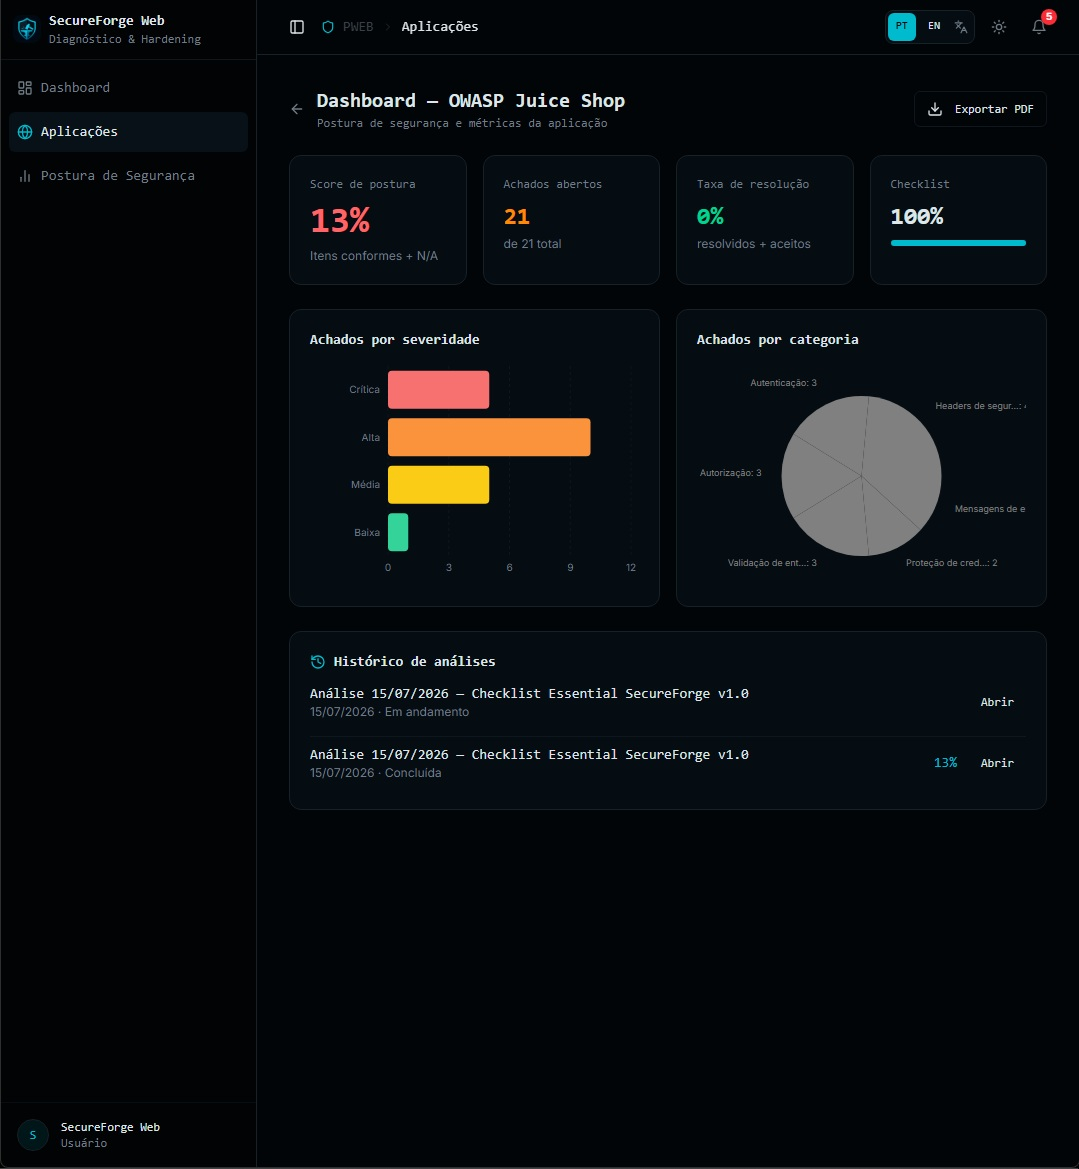
\includegraphics[width=0.95\linewidth]{fig-juice-dashboard.jpg}
  \caption{Dashboard da aplicação OWASP Juice Shop: score 13\%, 21 achados abertos, checklist 100\% e distribuição por severidade (5/10/5/1).}
  \label{fig:juice-dash}
\end{figure}

\begin{figure}[!ht]
  \centering
  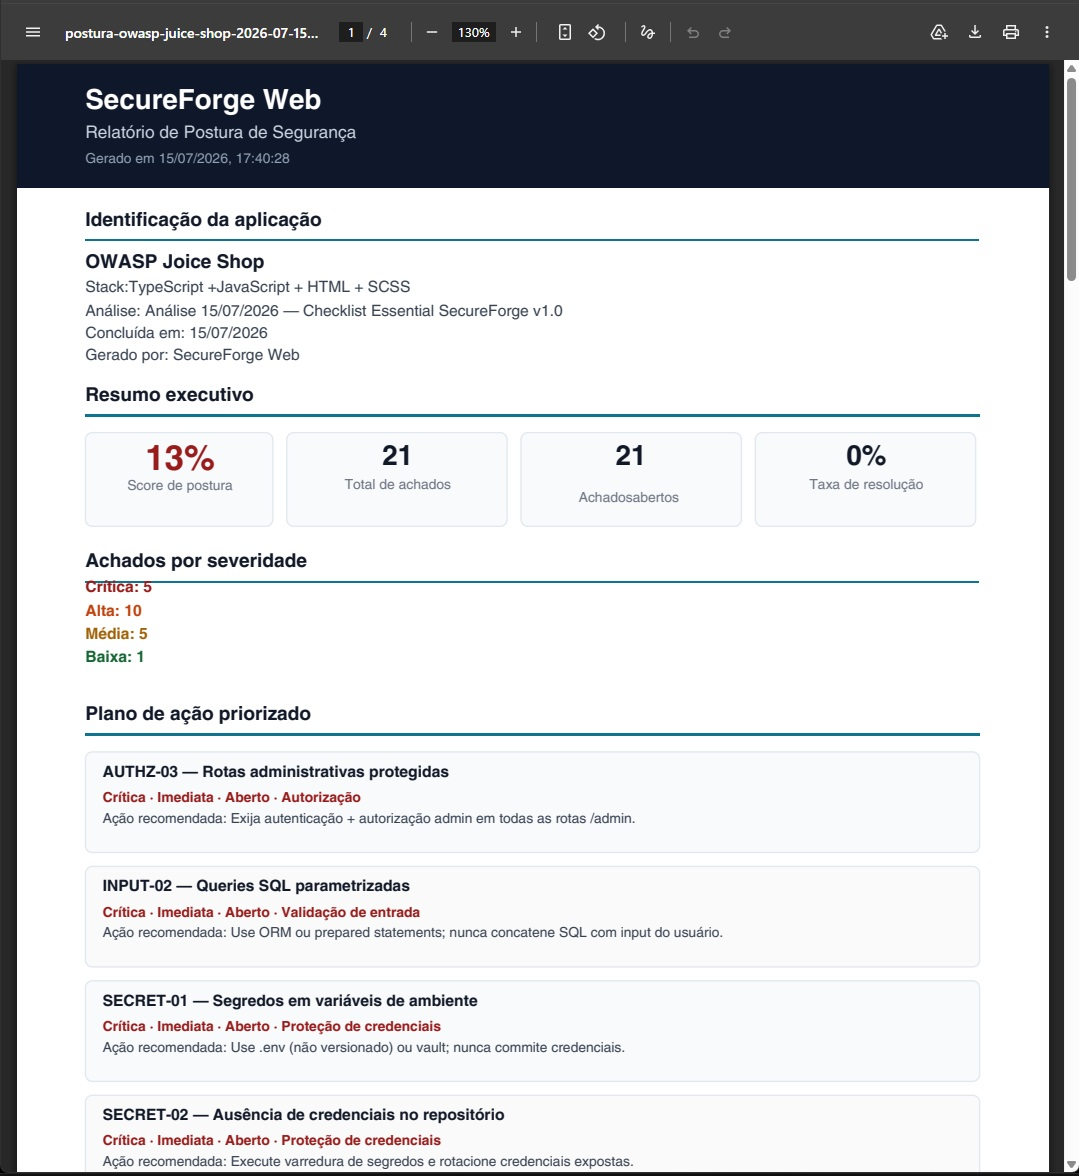
\includegraphics[width=0.85\linewidth]{fig-juice-pdf.jpg}
  \caption{Exemplo do PDF de postura gerado para o OWASP Juice Shop.}
  \label{fig:juice-pdf}
\end{figure}

A lista de achados registrou status operacional \emph{Aberto} para todos os 21 itens, com classificação de conformidade \emph{Não conforme} ou \emph{Parcialmente conforme}. O sistema emitiu notificações para achados críticos (5 alertas na interface). O assistente de IA (OpenAI \texttt{gpt-4o-mini}) foi configurado e validado antes da análise, permitindo sugestões assistidas por item/categoria e análise de repositório Git no \emph{wizard}.

\subsubsection{SecureForge Web (autoavaliação e hardening)}
A baseline (HTTP em Vite) resultou em \textbf{score de 29\%} e 17 achados (3 críticos: AUTH-02, AUTHZ-03, DATA-01). Com TLS local (\texttt{mkcert}) o score subiu para \textbf{42\%} (14 achados; críticos remanescentes: SECRET-01/02 e DATA-01 sob influência de URL/headers e fusão LLM). Após remediação focada nos itens críticos e altos --- headers Helmet/CSP/HSTS na API e no Vite, redação de logs, \texttt{escapeHtml}, fusão LLM que preserva evidências HTTP/Git de alta confiança, e cadastro da URL \texttt{https://localhost:3000} --- a reavaliação heurística HTTP+Git atingiu \textbf{score de 100\%} com \textbf{0 achados}. As Figuras~\ref{fig:sf-dash} e~\ref{fig:sf-findings} documentam o estado intermediário (pré-remediação completa) usado como evidência do fluxo diagnóstico.

\begin{figure}[!ht]
  \centering
  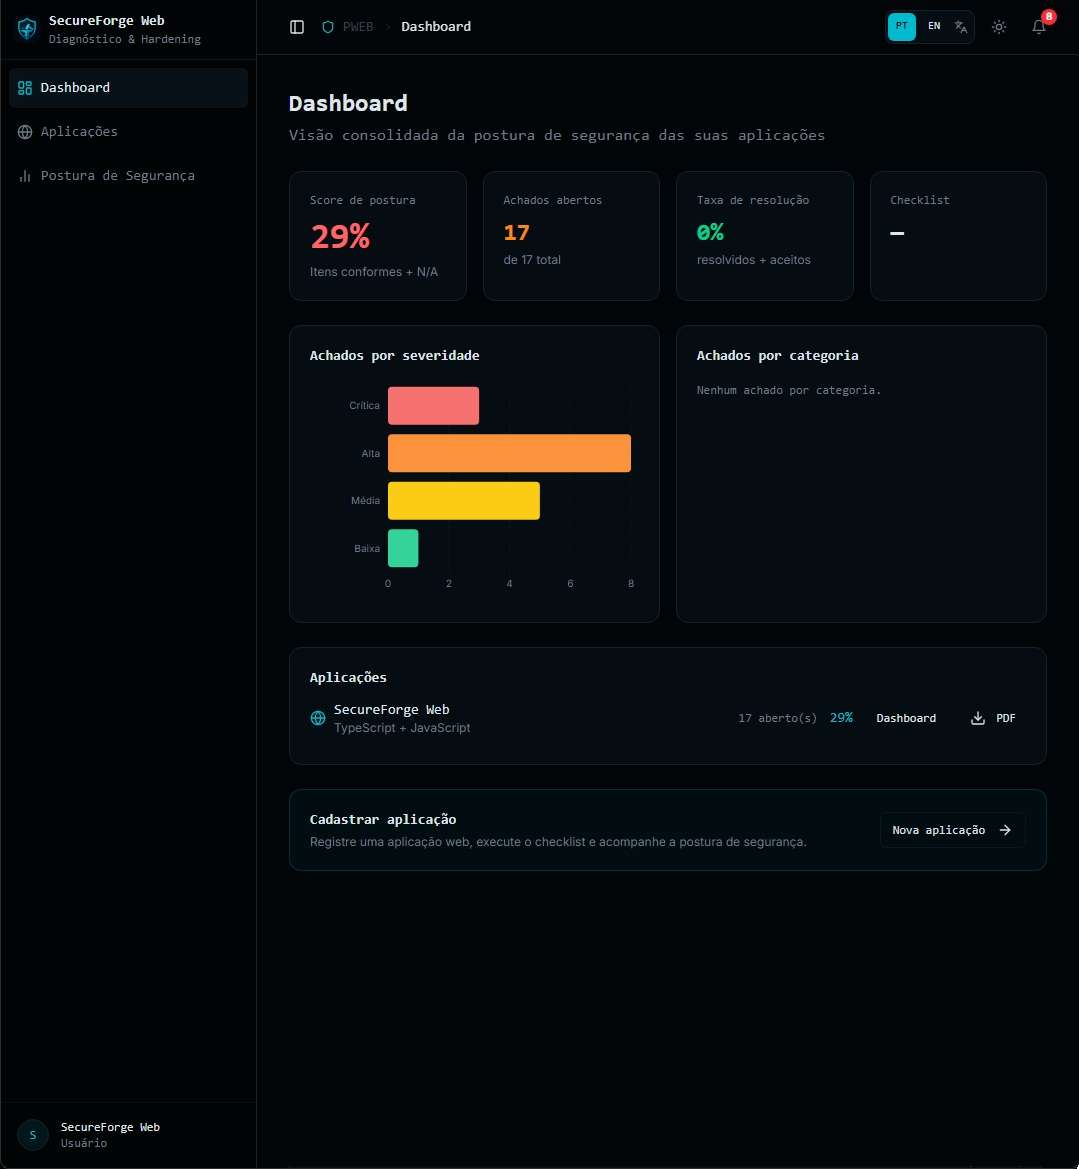
\includegraphics[width=0.95\linewidth]{fig-sf-dashboard-global.jpg}
  \caption{Dashboard consolidado da SecureForge Web no estágio intermediário (score 29\%, 17 achados, distribuição 3/8/5/1) --- evidência do ciclo diagnóstico antes do hardening completo.}
  \label{fig:sf-dash}
\end{figure}

\begin{figure}[!ht]
  \centering
  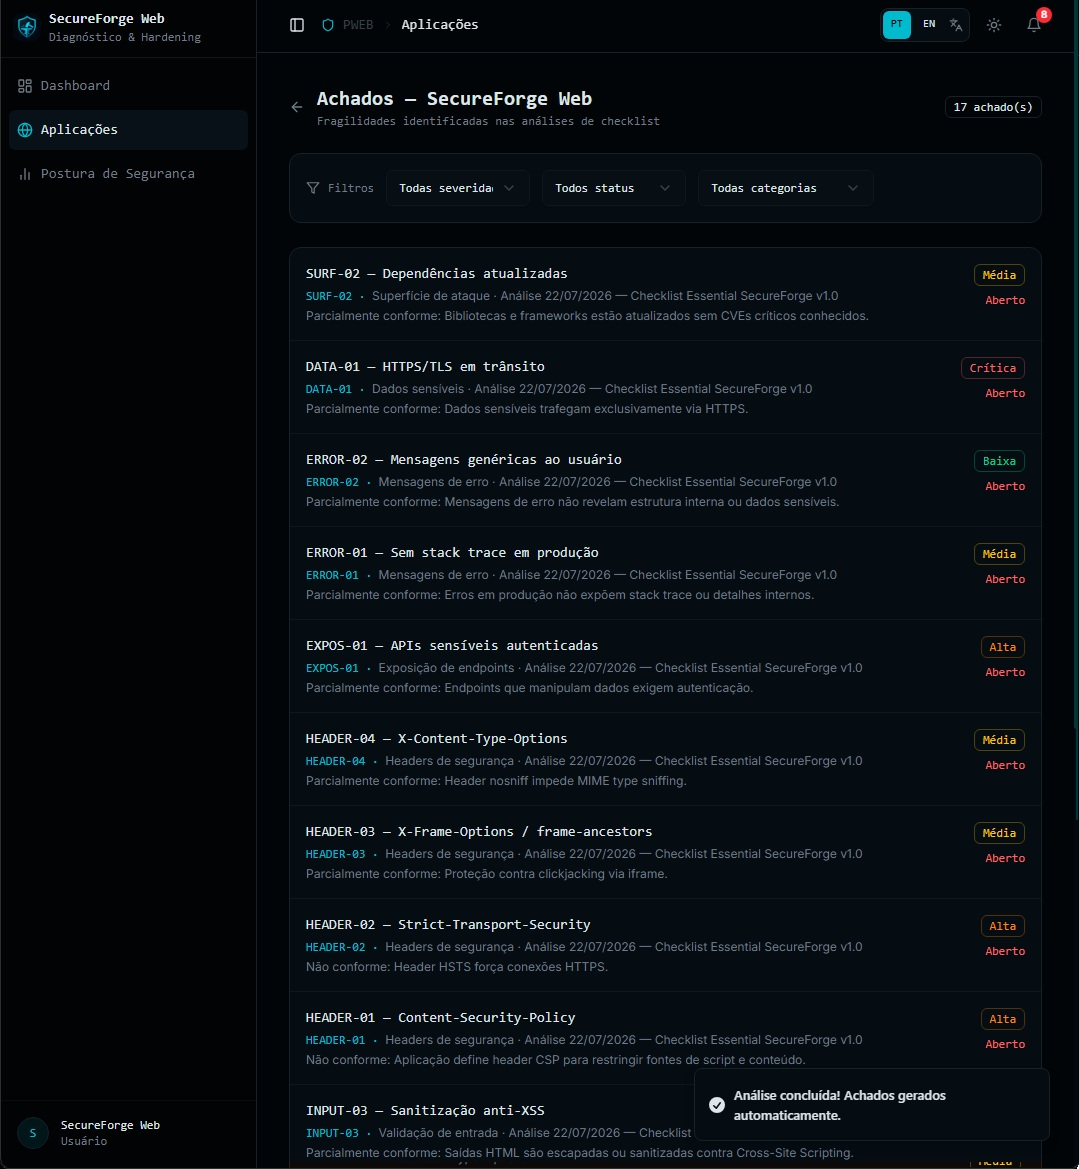
\includegraphics[width=0.95\linewidth]{fig-sf-findings.jpg}
  \caption{Lista de achados da SecureForge Web gerados automaticamente no estágio intermediário (toast de geração de achados).}
  \label{fig:sf-findings}
\end{figure}

\subsubsection{Exemplos de evidências por escopo}
A Tabela~\ref{tab:auth} resume exemplos qualitativos de sugestões e evidências na categoria Autenticação / Headers, conforme o comportamento dos assessores.

\begin{table}[!ht]
\centering
\caption{Exemplos de resultados por escopo de automação assistida.}
\label{tab:auth}
\begin{tabular}{p{1.4cm}p{1.4cm}p{2.2cm}p{4.8cm}}
\toprule
\textbf{Item} & \textbf{Escopo} & \textbf{Resultado} & \textbf{Evidência gerada} \\
\midrule
AUTH-01 & Git & Conforme & Política/validação de senha (Joi) \\
AUTH-02 & Git & Conforme & \texttt{bcrypt.hash} com custo 12 \\
HEADER-02 & HTTP & Conforme$^*$ & HSTS via Helmet na API HTTPS \\
DATA-01 & HTTP & Conforme$^*$ & Resposta final em HTTPS \\
Checklist & IA & 24 sugestões & Orquestração HTTP + Git + LLM (sem sobrescrever evidência forte) \\
\bottomrule
\end{tabular}
\end{table}
{\footnotesize $^*$Medição pós-hardening com URL \texttt{https://localhost:3000} (ou Vite HTTPS com sonda automática da API).}

O tempo de execução do assessor Git ficou tipicamente entre 15 e 45~s; a avaliação HTTP completou em menos de 12~s por URL; o assistente IA variou de poucos segundos (heurística) a dezenas de segundos (LLM com 24 itens); a geração do PDF concluiu em menos de 3~s. O fluxo ponta a ponta --- da criação da análise ao relatório --- foi executado sem intervenção manual no banco de dados, confirmando a integração entre camadas.

\subsection{Discussão}
Os resultados corroboram o posicionamento da ferramenta: (i)~em alvo intencionalmente vulnerável (Juice Shop), o score baixo e o volume de achados críticos/altos refletem a postura frágil esperada; (ii)~na autoavaliação, a SecureForge Web evoluiu de 29\% (HTTP) para 42\% (TLS) e, após remediação dos achados críticos/altos, para 100\% com evidências HTTP+Git; (iii)~a escolha da URL base (Vite vs.\ API) e a preservação de evidências automáticas frente ao LLM influenciam materialmente o score; (iv)~a persistência de evidências, notificações e PDF exportável materializam rastreabilidade útil para revisão humana e documentação acadêmica.

\section{Conclusão}
A SecureForge Web materializa a proposta da trilha AppHardener em ferramenta operacional: checklist OWASP guiado, automação assistida com três escopos complementares, evidências estruturadas por item e fluxo de \emph{hardening} com achados, postura e PDF. A avaliação experimental sobre Juice Shop e sobre a própria plataforma --- incluindo ciclo de remediação até score 100\% --- confirmou operação ponta a ponta e utilidade didática para equipes sem processo formal de AppSec.

Como trabalhos futuros, planeja-se: expandir cobertura de linguagens e \emph{frameworks} nas heurísticas Git; suportar repositórios privados com \emph{token}; integrar varredura de dependências (\texttt{npm audit}, OSV); incorporar comparação por categoria OWASP no \emph{benchmark}; e avaliar a ferramenta com múltiplas equipes em cenário controlado, medindo tempo de revisão e taxa de aceitação de sugestões automáticas.

\bibliographystyle{sbc}
\bibliography{references}

\end{document}
